\section{Methodology}
\label{sec:method}



\begin{figure}[t]
    \centering
    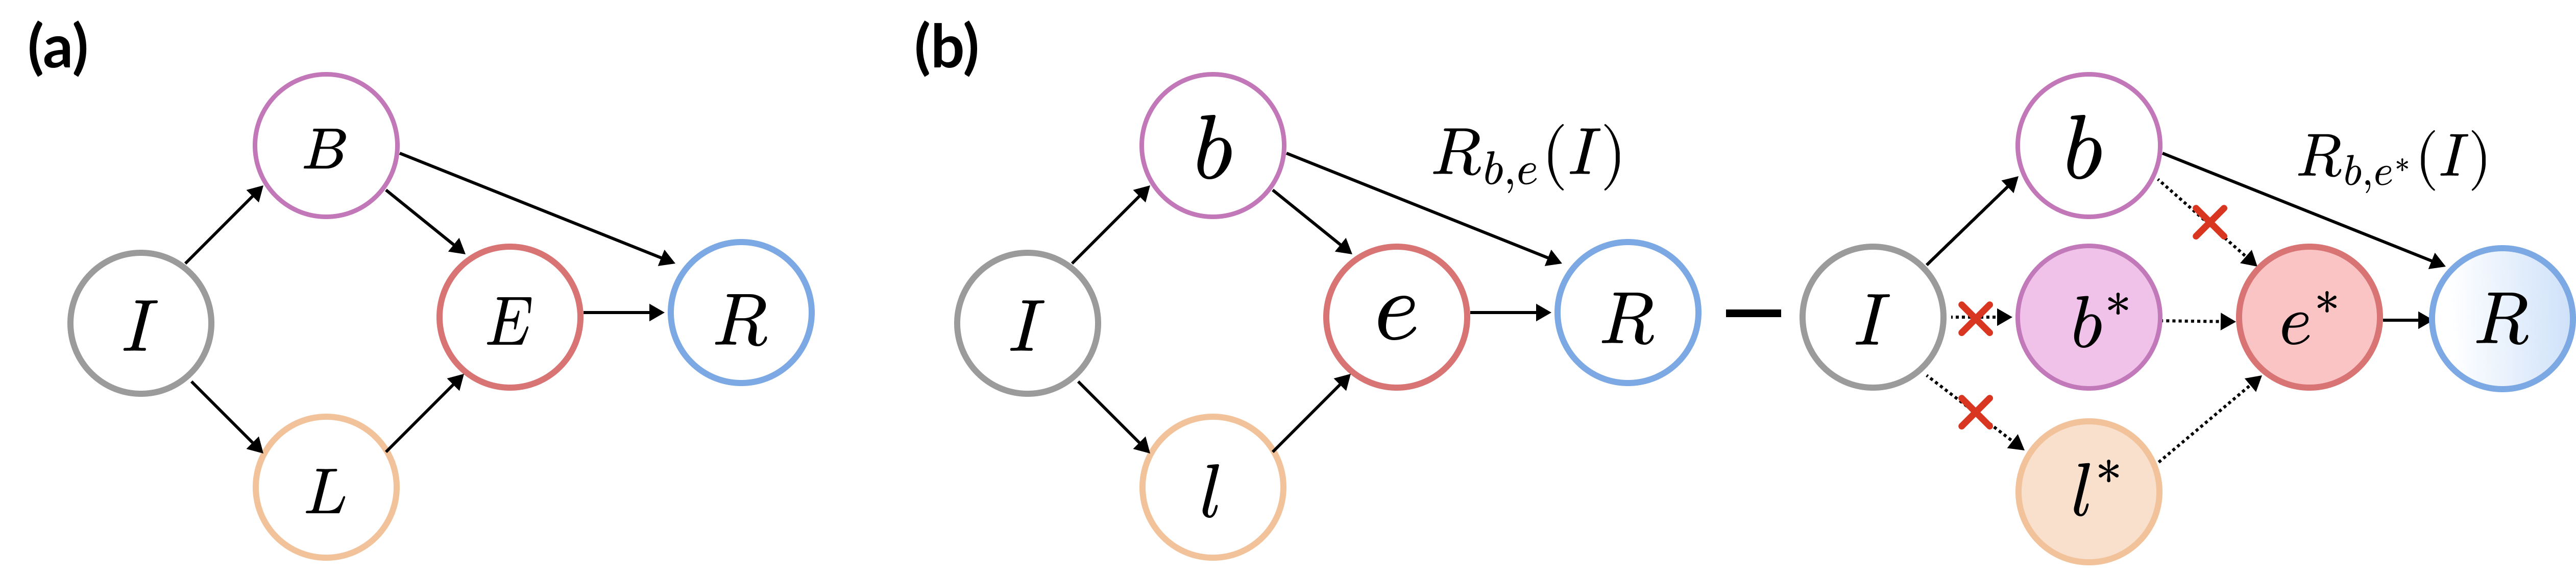
\includegraphics[width=0.45\textwidth]{figs/cvpr_fig3.png}
    \caption{Comparison between (a) SCM of Med-LVLM and (b) Counterfactual SCM of Med-LVLM.}
    \label{fig:scm}
\end{figure}

\subsection{Cause-Effect Look in Preference Optimization}
\subsubsection{Causal Analysis}
As illustrated in Fig. \ref{fig:scm}, the proposed causal graph for medical multimodal alignment consists of four key components: the medical image input $I$, its decomposed visual factors including the background $B$ and lesion evidence $L$, the learned joint features $E$, and the resulting reward model $R$. Based on the causal dependencies among these variables, we summarize the major links as follows.

\noindent\textbf{Link $I \rightarrow B \rightarrow R$} 
captures the harmful shortcut between the original input image and the reward through biased background correlations. Background factors $B$ (e.g., scanner type, imaging device, or patient posture) may be spuriously correlated with certain labels or textual descriptions, leading the model to achieve high reward even when clinically irrelevant regions dominate the decision \cite{zech2018variable}.

\noindent\textbf{Link $B \leftarrow I \rightarrow L$} depicts the generation of both background and lesion representations from the same medical image input. $I$ is processed by the visual encoder to produce background features $B$ and lesion features $L$ together. $B$ corresponds to global background such as lung field structure or imaging device signatures, while $L$ represents suspicious regions detected by attention or segmentation models.


\noindent\textbf{Link $B/L \rightarrow E \rightarrow R$.} captures the total causal influence of visual representations on the reward through the embedding $E$, which aggregates both background and lesion features learned from the visual encoder. In particular, $B$ provides the valuable contextual prior along the good causal link $B \rightarrow E \rightarrow R$, 
which facilitates reliable recognition when lesion information are subtle or visually confounded by surrounding anatomical structures. For example, in chest radiography, global contextual cues such as lung symmetry, cardiac silhouette, or diaphragm curvature help disambiguate faint opacities and improve diagnostic localization \cite{irvin2019chexpert}. This clinically grounded pathway allows CaMedPO to preserve meaningful joint information while mitigating harmful direct effects from $B$ on $R$.

\subsubsection{Causal Reward}

To isolate clinically meaningful signals from biased supervision, 
we model the causal effect of the background factor $B$ on the reward $R$ through the ensemble mediator $E$. 
Specifically, the factual reward generation process under a given input image $I$ can be expressed as:
\begin{equation}
R_{b,e}(I) = R(B=b, E_{b,l}=E(B=b,L=l) \mid I).
\end{equation}
The factual reward $R_{b,e}(I)$ inherently mixes both the useful lesion-grounded information and the harmful direct effect from $B$. 
To quantify these distinct contributions, we first define the Total Effect (TE) as:
\begin{equation}
\mathrm{TE} = R_{b,e}(I) - R_{b^{*},e^{*}}(I),
\end{equation}
where $b^{*}$ and $e^{*}$ correspond to the counterfactual background and its associated ensemble embedding. We next estimate the Natural Direct Effect (NDE) of $B$ for the pure harmful background bias:
\begin{equation}
\mathrm{NDE} = R_{b,e^{*}}(I) - R_{b^{*},e^{*}}(I).
\end{equation}
$R_{b,e^{*}}(I)$ denotes the counterfactual outcome: 
\begin{equation}
\small
R_{b,e^{*}}(I) = R(B=b, E_{b^{*},l^{*}}=E(B=b^{*},L=l^{*}) \mid I).
\end{equation}
As the indirect effect of embedding $E$ on the link $I \rightarrow B/L \rightarrow E \rightarrow R$ is blocked, the reward model can only be biased relying on the direct effect in the link $I \rightarrow B \rightarrow R$. To mitigate the background bias in NDE, we compute the Total Indirect Effect (TIE) by subtracting NDE from TE:
\begin{equation}
\mathrm{TIE} = R_{b,e}(I) - R_{b,e^{*}}(I).
\label{eq:tie}
\end{equation}
Intuitively, $\mathrm{TIE}$ represents the reward improvement driven by medically relevant background–lesion interactions.

\subsection{Theoretical Analysis}
\label{sec:theory}

To isolate clinically meaningful signals from biased supervision, we model the causal effect of the background factor $B$ on the reward $R$ through the ensemble mediator $E$.
Specifically, the factual reward generation process under a given input image $I$ can be expressed as:
\begin{equation}
|R_{b,e}(I) = R(B=b, E_{b,l}=E(B=b,L=l) \mid I).
\end{equation}

We define the causal reward contrast as:
\begin{equation}
    r_c(x,y) := R_{b,e}(x,y) - R_{b,e^*}(x,y).
    \label{eq:causal_reward_def}
\end{equation}

Under the assumption that the factual and counterfactual policies are latent KL-regularized MaxEnt optima, we substitute the reward-policy duality $R(x,y) = \eta^{-1} \log \frac{\pi(y \mid x)}{\pi_{\text{ref}}(y \mid x)} + \eta^{-1} \log Z(x)$ into Eq. \ref{eq:causal_reward_def}. The partition functions $Z(\cdot)$ cancel out in the pairwise difference, directly yielding the log-likelihood difference form used in our objective. This derivation relies on the assumption that fitting the same optimized policy $\pi_{\theta}$ provides a consistent surrogate for the causal reward contrast.

In standard DPO, the optimization is based on the relative preference difference 
between a preferred sample $y_w$ and a dispreferred one $y_l$, where the reward difference $r(x,y_w)-r(x,y_l)$ determines the training direction. However, such rewards may still encode background-related biases that affect both positive and negative samples. To obtain a bias-free causal preference, we define the conventional reward $r$ 
with the total indirect effect $r_\text{TIE}$ as expressed in Eq. \ref{eq:tie}. Substituting $r_{\text{TIE}}$ into the Bradley--Terry model, the preference probability between $(y_w,y_l)$ becomes
\begin{equation}
P(y_w \succ y_l \mid x)
= \sigma\!\left(\eta\,[\,r_{c}(x,y_w)-r_{c}(x,y_l)\,]\right),
\end{equation}
where $\sigma(\cdot)$ is the logistic function. 
The difference $r_{c}(x,y_w)-r_{c}(x,y_l)$ serves as a \textit{causal contrast} that reflects the pure clinical contribution through the mediator $E$. Expanding this difference yields

\begin{equation}
\small
\begin{aligned}
    r_{c}(x,y_w)-r_{c}(x,y_l)
= \underbrace{[R_{b,e}(x,y_w)-R_{b,e}(x,y_l)]}_{\text{factual difference}}
 &\\-\underbrace{[R_{b,e^*}(x,y_w)-R_{b,e^*}(x,y_l)]}_{\text{counterfactual difference}}.
\end{aligned} 
\label{eq:preference}
\end{equation}
This symmetric structure indicates that both the positive and negative samples 
are corrected by the same causal mechanism.  
If the correction were applied only to the preferred response $y_w$, 
the residual background effect on $y_l$ would remain, 
and the pairwise reward difference would still contain the direct bias from $B$. 

In preference optimization, the reference policy
$\pi_{\text{ref}}$ is typically obtained from a supervised fine-tuned (SFT) model that aligns to instruction-following data. However, $\pi_{\text{ref}}$ may carry bias from the underlying training distribution, causing modality shortcuts in medical preference learning. Our goal is to show that the proposed optimization goal can theoretically correct these biases and converge to a causal-optimal policy. Formally, we define the causal-optimal policy and provide a convergence guarantee based on the unbiased TIE reward. Let $\pi_{\text{ref}}$ be an arbitrary reference policy. The observed reward can be decomposed as
\[
r_o(x,y) \;=\; r_c(x,y) + \delta(x,y),
\]
where $r_c$ is the causal TIE reward
and $\delta$ denotes the bias caused by the direct background effect.
Assume all rewards are bounded by $|r_c|,|\delta|\le R_{\max}$.

\begin{definition}[Causal-optimal policy]
\label{def:causal_optimal}
Given a biased reference policy $\pi_{\text{ref}}$ and the unbiased
TIE reward $r_c(x,y)=R_{b,e}(I)-R_{b,e^*}(I)$,
the \emph{causal-optimal policy} is defined as
\[
\pi_c^\star(y \mid x)
\propto
\pi_{\text{ref}}(y \mid x)
\exp\!\big(\eta\,r_c(x,y)\big).
\]
\end{definition}

\begin{theorem}[Convergence of causal reward]
\label{thm:tie_convergence}
Under Assumption~\ref{ass:bounded} that all rewards are bounded by
$R_{\max}$, the bias magnitude satisfies $\|\delta\|_\infty \le \varepsilon$,
and the learning rate $\eta$ is sufficiently small,
the policy sequence updated by TIE-DPO satisfies
\[
\small
\begin{aligned}
\mathbb{E}\!\big[
\mathrm{KL}(\pi_{T+1}\|\pi_c^\star)
\big]
&\le
\mathrm{KL}(\pi_1\|\pi_c^\star)
-\eta
\sum_{t=1}^{T}
\mathbb{E}_{x,e}\!\big[
\mathrm{Var}_{\pi_t}(r_c)
\big]  \\
&\quad
+\,O(T\eta^2R_{\max}^2).
\end{aligned}
\]
which ensures a monotonic improvement toward the causal-optimal
policy $\pi_c^\star$.
\end{theorem}

\noindent
The bias term $\delta$ amplifies spurious correlations between background and reward, 
causing the exponentiated policy update to deviate from the causal optimum. Full derivations and proofs are provided in Appendix \ref{supp:theory}.

\begin{figure*}[!htbp]
    \centering
    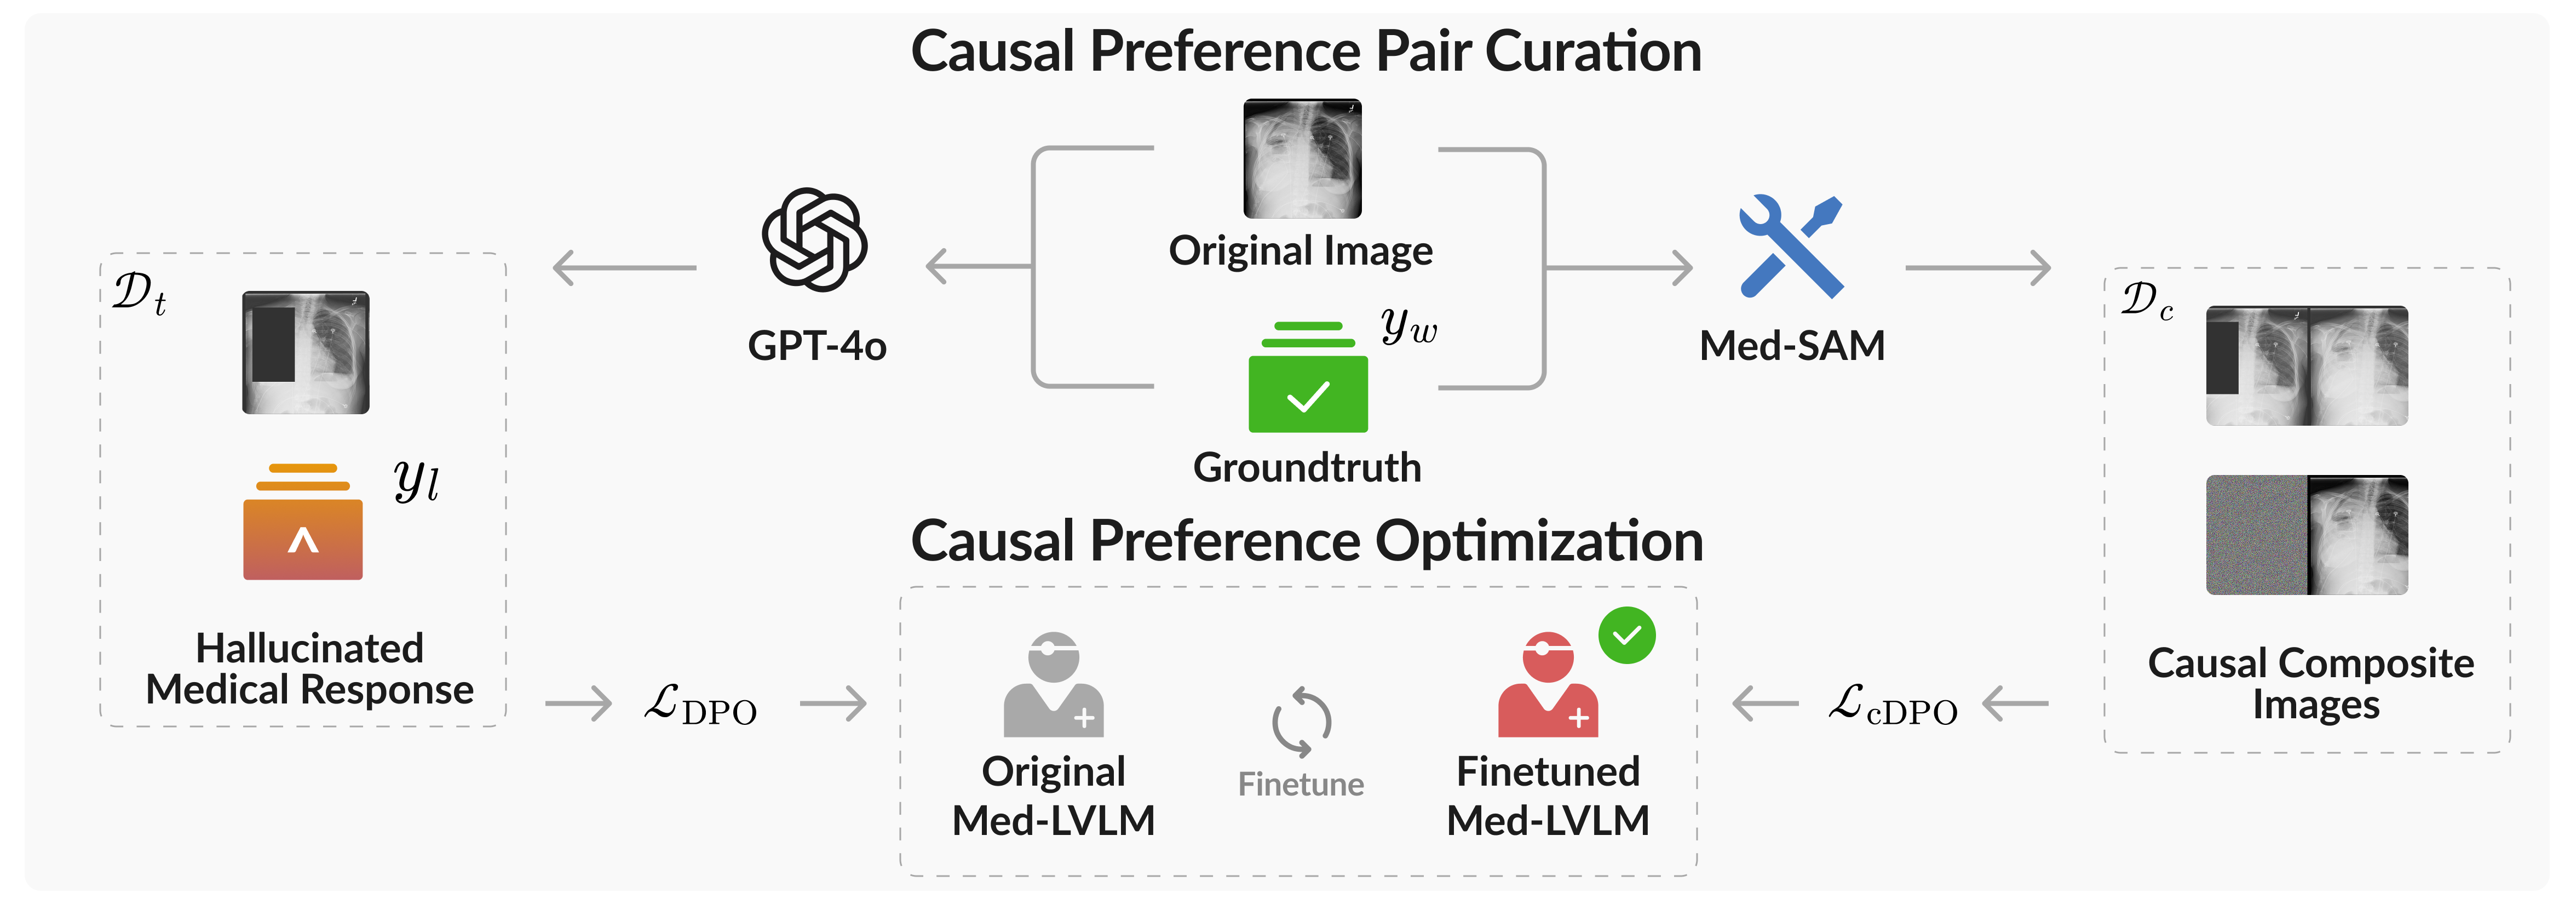
\includegraphics[width=0.9\textwidth]{figs/cvpr_fig4.png}
    \caption{The overview of CaMedPO that consists of the causal preference pair curation and causal preference optimization.}
    \label{fig:structure}
\end{figure*}

\subsection{Implementation Instantiation}


\subsubsection{Causal Preference Pair Curation}
To realize the causal preference structure defined in Eq. \ref{eq:preference}, we curate paired data that reflect both factual and counterfactual medical reasoning, where the whole framework is illustrated in Fig. \ref{fig:structure}. The construction proceeds in two stages.

\textbf{Generating Hallucinated Medical Responses.}
Following the causal contrastive formulation, we first obtain dispreference responses $\!y_l\!$ by introducing factual inconsistencies into medical reports, following the approach in MMedPO \cite{Zhu2025MMedPO}. Specifically, we employ GPT-4o \cite{achiam2023gpt} to generate multiple candidate responses for each case sampled from the target Med-LVLMs, and evaluate their factual consistency against the ground-truth response $y_w$. The candidate exhibiting the highest hallucination score, such as incorrect image interpretation or misleading diagnostic reasoning, is selected as the dispreference response. When no candidate response exhibits sufficient deviation, GPT-4o is prompted to synthesize a dispreference response. The preference pairs constructed by this process are denoted as $\mathcal{D}_t$.


\textbf{Constructing Causal Composite Images.}
To explicitly instantiate the causal mechanism illustrated in our causal graph, we construct composite visual inputs that allow controlled intervention on lesion and background evidence. Specifically, we employ a medical visual localization tool to segment the lesion area from the original image $I$, identifying the regions most relevant to disease diagnosis. The lesion mask is then removed, and the masked region is filled with zero-valued pixels to form a background-only image $I_b$, representing the background variable $B{=}b$ in the structural causal model. The original image $I$ serves as the factual visual condition associated with the denoted $E{=}e$, while a Gaussian noise-perturbed version of the same image serves as the counterfactual condition $E{=}e^*$.

To construct counterfactual inputs, we stitch background-only images with noise-perturbed originals. While this introduces artificial boundaries, our results (Table \ref{tab:causal_validation}) show that the model learns the intended causal contrast rather than overfitting to stitching artifacts, as performance remains robust on standard clean images.

These components are combined into composite image pairs that preserve the same anatomical context but differ in the lesion evidence, forming the factual and counterfactual visual conditions: $(I_b \oplus I) \quad \text{and} \quad (I_b \oplus I_{\text{null}})$, where $\oplus$ denotes image stitching. Each pair is associated with a clinical query prepended by an instruction emphasizing that both images come from the same patient, such as “\textit{Both images belong to the same patient. Please analyze each and then provide a joint clinical conclusion}”, where the revised clinical query is denoted as $T'$. The preference data constructed in this stage is denoted as $\mathcal{D}_c$. By aligning the composite inputs with their preferred and dispreference textual responses, we obtain the overall preference dataset $\mathcal{D}_f = \mathcal{D}_t \cup \mathcal{D}_c = 
\big\{(x^{(i)},x^{*(i)},x_c^{(i)},x_c^{*(i)},y_w^{(i)},y_l^{(i)})\big\}_{i=1}^N$,
where $x^{(i)}=(I,T)$ and $x^{*(i)}=(I_b,T)$ are the standard preference pairs used in MMedPO, while $x_c^{(i)}=(I_b\!\oplus\!I,T')$ and $x_c^{*(i)}=(I_b\!\oplus\!I_{\text{null}},T')$ are the causal pairs.

\subsubsection{Causal Preference Optimization}
Changing $R$ with its logarithmic likelihood form used in DPO, we obtain the causal logit
\begin{equation}
\small
\begin{aligned}
\Lambda_{\text{cDPO}}
&=\Big[
\log \frac{\pi_\theta(y_w \mid x_c)}{\pi_{\text{ref}}(y_w \mid x_c)}
-\log \frac{\pi_\theta(y_w \mid x_c^*)}{\pi_{\text{ref}}(y_w \mid x_c^*)}
\Big]  \\
&\quad -
\Big[
\log \frac{\pi_\theta(y_l \mid x_c)}{\pi_{\text{ref}}(y_l \mid x_c)}
-\log \frac{\pi_\theta(y_l \mid x_c^*)}{\pi_{\text{ref}}(y_l \mid x_c^*)}
\Big].
\end{aligned}
\end{equation} Therefore, the causal optimization objective is
\begin{equation}
\mathcal{L}_{\text{cDPO}}
= -\mathbb{E}_{(x_c,x_c^*,y_w,y_l)\sim\mathcal{D}_f}
  \left[\log\sigma\!\big(\eta^{-1}\Lambda_{\text{cDPO}}\big)\right],
\end{equation}
Note that the original MMedpo preference optimization goal is also retrained to keep the Med-LVLM has the ability to make predictions according to the original visual and clinical query inputs. The optimization objective is
\begin{equation}
\small
\begin{aligned}
&\mathcal{L}_{\text{DPO}} = -\mathbb{E}_{(x,x^*,y_w,y_l)\sim\mathcal{D}_f} \\
&\Bigg[
\log \sigma \Big(
\eta^{-1} \log \frac{\pi_\theta(y_w|x)}{\pi_{\text{ref}}(y_w|x)}
- \eta^{-1} \log \frac{\pi_\theta(y_l|x^*)}{\pi_{\text{ref}}(y_l|x^*)}
\Big) \Bigg].
\end{aligned}
\end{equation} However, we do not employ the clinical relevance score used in MMedPO to reduce the computational workload. Finally, the objective of CaMedPO is the combination of the two preference optimizations:
\begin{equation} \mathcal{L}_\text{CaMedPO}=\mathcal{L}_{\text{DPO}}+\mathcal{L}_{\text{cDPO}}.
\label{eq:final_loss}
\end{equation}





